\documentclass[11pt,a4paper]{article}
\usepackage[T1]{fontenc}
\usepackage[utf8]{inputenc}
\usepackage{lmodern}
\usepackage[varqu,scaled=0.95]{zi4}
\usepackage[margin=2.3cm,headheight=14pt]{geometry}
\usepackage{microtype}
\usepackage{graphicx}
\usepackage{booktabs}
\usepackage{tabularx}
\usepackage{amsmath,amssymb}
\usepackage{float}
\usepackage{placeins}
\usepackage{needspace}
\usepackage{xcolor}
\usepackage[parfill]{parskip}
\usepackage{enumitem}
\usepackage{titlesec}
\usepackage{fancyhdr}
\usepackage[font=small,labelfont={bf,color=accent},skip=6pt]{caption}
\usepackage{listings}
\usepackage[most]{tcolorbox}
\usepackage[colorlinks=true,linkcolor=accent,citecolor=accent,urlcolor=accent]{hyperref}

% ---------------------------------------------------------------------
% Colours (methods match the figures)
\definecolor{accent}{HTML}{1F3A5F}
\definecolor{accentlight}{HTML}{EEF3F9}
\definecolor{rulegray}{HTML}{C9D3DF}
\definecolor{codebg}{HTML}{F8F9FB}
\definecolor{codekw}{HTML}{8A3FA0}
\definecolor{codecomment}{HTML}{6B7785}
\definecolor{mijk}{HTML}{2A78D6}
\definecolor{mikj}{HTML}{EB6834}
\definecolor{mtransposed}{HTML}{1BAF7A}
\definecolor{mblocked}{HTML}{4A3AA7}
\definecolor{mcsr}{HTML}{D4357A}

% ---------------------------------------------------------------------
% Headings
\titleformat{\section}{\Needspace{8\baselineskip}\Large\bfseries\color{accent}}{\thesection}{0.7em}{}
  [\vspace{-4pt}{\color{rulegray}\titlerule[0.8pt]}]
\titlespacing*{\section}{0pt}{18pt}{10pt}
\titleformat{\subsection}{\Needspace{7\baselineskip}\large\bfseries\color{accent}}{\thesubsection}{0.6em}{}
\titlespacing*{\subsection}{0pt}{14pt}{6pt}

% A concept heading on its own line, with space above, inside a section
\newcommand{\concept}[1]{\par\addvspace{8pt}\Needspace{5\baselineskip}%
  \noindent{\color{accent}\bfseries\boldmath #1}\par\nopagebreak\vspace{2pt}}

% Page style
\pagestyle{fancy}
\fancyhf{}
\fancyhead[L]{\small\color{codecomment}Assignment 2 \textperiodcentered{} Optimised dense and sparse matrix multiplication}
\fancyhead[R]{\small\color{codecomment}\AuthorName}
\fancyfoot[C]{\small\thepage}
\renewcommand{\headrulewidth}{0.4pt}
\renewcommand{\headrule}{{\color{rulegray}\hrule height\headrulewidth}}

% Lists
\setlist{itemsep=3pt,parsep=0pt,topsep=4pt}

% Floats: let large figures and tables share pages with text instead of leaving gaps
\renewcommand{\topfraction}{0.85}
\renewcommand{\bottomfraction}{0.6}
\renewcommand{\textfraction}{0.1}
\renewcommand{\floatpagefraction}{0.8}
\setcounter{topnumber}{3}
\setcounter{totalnumber}{4}

% ---------------------------------------------------------------------
% Boxes
\newtcolorbox{infobox}[1][]{enhanced,breakable,colback=accentlight,colframe=accent,
  boxrule=0pt,leftrule=3pt,arc=0pt,left=10pt,right=10pt,top=6pt,bottom=6pt,
  before upper={\setlength{\parskip}{5pt}},#1}
\newtcolorbox{titledbox}[1]{enhanced,breakable,colback=accentlight,colframe=accent,
  boxrule=0.6pt,arc=2pt,left=10pt,right=10pt,top=6pt,bottom=6pt,
  title={\bfseries #1},fonttitle=\normalsize,coltitle=white,
  before upper={\setlength{\parskip}{5pt}}}

% Code listings
\lstdefinestyle{kernel}{
  basicstyle=\ttfamily\small,
  keywordstyle=\color{codekw}\bfseries,
  commentstyle=\color{codecomment}\itshape,
  stringstyle=\color{codecomment},
  numbers=left, numberstyle=\scriptsize\color{codecomment}, numbersep=8pt,
  showstringspaces=false, columns=fullflexible, keepspaces=true,
  aboveskip=0pt, belowskip=0pt, xleftmargin=14pt
}
\newtcblisting{codebox}[3]{enhanced,breakable,listing only,
  listing options={style=kernel,language=#1},
  colback=codebg,colframe=#3,boxrule=0.6pt,leftrule=3pt,arc=2pt,
  left=4pt,right=6pt,top=4pt,bottom=4pt,
  title={\ttfamily\small #2},coltitle=black,colbacktitle=#3!12,
  fonttitle=\bfseries,toptitle=1pt,bottomtitle=1pt}

% Tables
\renewcommand{\arraystretch}{1.12}

% ---------------------------------------------------------------------
% Generated by scripts/analyze.py -- do not edit by hand.
\newcommand{\DenseTimeTable}{
\begin{tabular}{r r r r r r r r r }\toprule
& \multicolumn{2}{c}{ijk} & \multicolumn{2}{c}{ikj} & \multicolumn{2}{c}{transposed} & \multicolumn{2}{c}{blocked} \\\cmidrule(lr){2-3}\cmidrule(lr){4-5}\cmidrule(lr){6-7}\cmidrule(lr){8-9}
$n$ & Median & IQR\% & Median & IQR\% & Median & IQR\% & Median & IQR\% \\\midrule
64 & 142.8 $\mu$s & 4.0 & 56.6 $\mu$s & 9.6 & 156.8 $\mu$s & 7.7 & 50.7 $\mu$s & 10.8 \\
128 & 2.96 ms & 4.5 & 346.8 $\mu$s & 8.8 & 1.28 ms & 5.9 & 427.7 $\mu$s & 4.2 \\
256 & 34.12 ms & 0.9 & 3.37 ms & 7.6 & 11.48 ms & 3.6 & 3.33 ms & 8.5 \\
512 & 373.56 ms & 1.9 & 27.76 ms & 24.4 & 98.04 ms & 2.3 & 30.22 ms & 2.2 \\
768 & 1.05 s & 0.4 & 96.04 ms & 18.0 & 336.81 ms & 1.5 & 85.75 ms & 35.2 \\
1024 & 5.93 s & 0.6 & 225.96 ms & 26.2 & 799.79 ms & 2.2 & 222.61 ms & 1.7 \\
1536 & 18.24 s & 0.4 & 1.44 s & 1.0 & 2.82 s & 0.2 & 760.86 ms & 10.2 \\
2048 & 49.02 s & 0.5 & 3.42 s & 0.6 & 6.74 s & 0.0 & 1.76 s & 3.6 \\
3072 & 182.04 s & 0.5 & 12.83 s & 0.7 & 22.92 s & 0.1 & 5.72 s & 0.7 \\
4096 & \multicolumn{2}{c}{\textit{timeout}} & 29.36 s & 0.4 & 54.53 s & 0.3 & 13.89 s & 1.7 \\
\bottomrule\end{tabular}}
\newcommand{\DenseSpeedupTable}{
\begin{tabular}{r r r r r r r r r r}\toprule
& \multicolumn{3}{c}{Speed-up over ijk} & \multicolumn{4}{c}{GFLOP/s ($2n^3$/median)} & \multicolumn{2}{c}{Peak WS (MB)} \\\cmidrule(lr){2-4}\cmidrule(lr){5-8}\cmidrule(lr){9-10}
$n$ & ikj & transp. & blocked & ijk & ikj & transp. & blocked & ijk & transp. \\\midrule
64 & 2.5 & 0.9 & 2.8 & 3.67 & 9.27 & 3.34 & 10.33 & 4 & 4 \\
128 & 8.5 & 2.3 & 6.9 & 1.42 & 12.09 & 3.28 & 9.81 & 4 & 5 \\
256 & 10.1 & 3.0 & 10.3 & 0.98 & 9.96 & 2.92 & 10.09 & 6 & 6 \\
512 & 13.5 & 3.8 & 12.4 & 0.72 & 9.67 & 2.74 & 8.88 & 10 & 12 \\
768 & 10.9 & 3.1 & 12.2 & 0.86 & 9.43 & 2.69 & 10.56 & 18 & 23 \\
1024 & 26.2 & 7.4 & 26.6 & 0.36 & 9.50 & 2.69 & 9.65 & 29 & 38 \\
1536 & 12.6 & 6.5 & 24.0 & 0.40 & 5.02 & 2.57 & 9.53 & 61 & 80 \\
2048 & 14.3 & 7.3 & 27.8 & 0.35 & 5.02 & 2.55 & 9.74 & 105 & 138 \\
3072 & 14.2 & 7.9 & 31.8 & 0.32 & 4.52 & 2.53 & 10.14 & 231 & 306 \\
4096 & -- & -- & -- & -- & 4.68 & 2.52 & 9.90 & -- & 541 \\
\bottomrule\end{tabular}}
\newcommand{\BlockSweepTable}{
\begin{tabular}{r r r r r r }\toprule $n$ & $b=16$ & $b=32$ & $b=64$ & $b=128$ & $b=256$ \\\midrule
512 & 38.25 ms & 28.25 ms & 25.41 ms & \textbf{24.56 ms} & 37.04 ms \\
1024 & 305.32 ms & 232.09 ms & \textbf{194.19 ms} & 240.59 ms & 268.84 ms \\
2048 & 2.69 s & 1.85 s & \textbf{1.62 s} & 2.03 s & 2.24 s \\
\bottomrule\end{tabular}}
\newcommand{\VecTable}{
\begin{tabular}{l r r r r}\toprule Method & $n$ & -O2 (SSE2 vectorised) & -O2 -fno-tree-vectorize & Ratio \\\midrule
ikj & 256 & 3.38 ms & 5.56 ms & 1.65$\times$ \\
ikj & 512 & 27.91 ms & 44.43 ms & 1.59$\times$ \\
ikj & 1024 & 256.26 ms & 329.66 ms & 1.29$\times$ \\
ikj & 2048 & 3.31 s & 4.14 s & 1.25$\times$ \\
\addlinespace[2pt]
blocked & 256 & 3.09 ms & 5.29 ms & 1.71$\times$ \\
blocked & 512 & 27.67 ms & 44.05 ms & 1.59$\times$ \\
blocked & 1024 & 192.85 ms & 322.15 ms & 1.67$\times$ \\
blocked & 2048 & 1.64 s & 2.65 s & 1.62$\times$ \\
\addlinespace[2pt]
transposed & 256 & 11.59 ms & 11.60 ms & 1.00$\times$ \\
transposed & 512 & 96.01 ms & 99.95 ms & 1.04$\times$ \\
transposed & 1024 & 795.54 ms & 794.73 ms & 1.00$\times$ \\
transposed & 2048 & 6.70 s & 6.71 s & 1.00$\times$ \\
\addlinespace[2pt]
\bottomrule\end{tabular}}
\newcommand{\VecChecksumsEqual}{yes}
\newcommand{\SparseTable}{
\begin{tabular}{r r r r r r r r r r}\toprule
$n$ & Dens.\,\% & nnz(A) & nnz(C) & Out dens.\,\% & CSR mult. & + conversions & Blocked & ijk & Speed-up$^\dagger$ \\\midrule
1024 & 0.1 & 1\,049 & 1\,123 & 0.107 & 8.8 $\mu$s & 3.68 ms & 231.57 ms & 4.15 s & 26\,250$\times$ \\
1024 & 0.5 & 5\,243 & 26\,628 & 2.54 & 192.6 $\mu$s & 4.45 ms & 218.31 ms & 4.02 s & 1\,134$\times$ \\
1024 & 1 & 10\,486 & 101\,969 & 9.72 & 471.6 $\mu$s & 5.27 ms & 222.57 ms & 4.98 s & 472$\times$ \\
1024 & 2 & 20\,972 & 352\,086 & 33.6 & 3.23 ms & 9.38 ms & 221.75 ms & 5.56 s & 68.7$\times$ \\
1024 & 5 & 52\,429 & 967\,449 & 92.3 & 18.13 ms & 25.45 ms & 244.92 ms & 5.53 s & 13.5$\times$ \\
1024 & 10 & 104\,858 & 1\,048\,540 & 100 & 31.31 ms & 40.11 ms & 209.29 ms & 5.64 s & 6.69$\times$ \\
1024 & 25 & 262\,144 & 1\,048\,576 & 100 & 131.29 ms & 144.95 ms & 215.05 ms & 4.91 s & 1.64$\times$ \\
1024 & 50 & 524\,288 & 1\,048\,576 & 100 & 410.17 ms & 432.79 ms & 223.28 ms & 5.25 s & 0.544$\times$ \\
1024 & 100 & 1\,048\,576 & 1\,048\,576 & 100 & 1.51 s & 1.52 s & 253.11 ms & 5.22 s & 0.168$\times$ \\
\addlinespace[3pt]
2048 & 0.1 & 4\,194 & 8\,673 & 0.207 & 102.3 $\mu$s & 18.73 ms & 1.74 s & -- & 16\,985$\times$ \\
2048 & 0.5 & 20\,972 & 209\,270 & 4.99 & 1.31 ms & 19.06 ms & 1.74 s & -- & 1\,324$\times$ \\
2048 & 1 & 41\,943 & 776\,382 & 18.5 & 5.52 ms & 26.66 ms & 1.77 s & -- & 320$\times$ \\
2048 & 2 & 83\,886 & 2\,346\,584 & 55.9 & 31.48 ms & 54.42 ms & 1.77 s & -- & 56.1$\times$ \\
2048 & 5 & 209\,715 & 4\,169\,706 & 99.4 & 99.55 ms & 129.83 ms & 1.71 s & -- & 17.2$\times$ \\
2048 & 10 & 419\,430 & 4\,194\,304 & 100 & 203.18 ms & 242.80 ms & 1.74 s & -- & 8.57$\times$ \\
2048 & 25 & 1\,048\,576 & 4\,194\,304 & 100 & 889.11 ms & 950.11 ms & 1.73 s & -- & 1.95$\times$ \\
2048 & 50 & 2\,097\,152 & 4\,194\,304 & 100 & 3.38 s & 3.47 s & 1.77 s & -- & 0.522$\times$ \\
2048 & 100 & 4\,194\,304 & 4\,194\,304 & 100 & 12.48 s & 12.53 s & 1.71 s & -- & 0.137$\times$ \\
\addlinespace[3pt]
\bottomrule\end{tabular}}
\newcommand{\SparseCostTable}{
\begin{tabular}{r r r r r r r r r r}\toprule
& & \multicolumn{3}{c}{CSR time (median)} & & \multicolumn{3}{c}{Peak WS (MB)} & Model (MB) \\\cmidrule(lr){3-5}\cmidrule(lr){7-9}\cmidrule(lr){10-10}
$n$ & Dens.\,\% & A,B$\to$CSR & Multiply & C$\to$dense & ns/product & CSR$^\ast$ & CSR only & Blocked & CSR $A,B,C$ \\\midrule
1024 & 0.1 & 2.66 ms & 8.8 $\mu$s & 1.01 ms & 7.86 & 21 & 4.1 & 29 & 0.1 \\
1024 & 0.5 & 2.84 ms & 192.6 $\mu$s & 1.42 ms & 7.14 & 22 & 4.5 & 29 & 0.5 \\
1024 & 1 & 3.22 ms & 471.6 $\mu$s & 1.58 ms & 4.40 & 23 & 5.6 & 29 & 1.5 \\
1024 & 2 & 4.05 ms & 3.23 ms & 2.10 ms & 7.53 & 26 & 8.8 & 29 & 4.8 \\
1024 & 5 & 4.82 ms & 18.13 ms & 2.50 ms & 6.76 & 35 & 17.0 & 30 & 12.9 \\
1024 & 10 & 6.26 ms & 31.31 ms & 2.54 ms & 2.92 & 38 & 19.2 & 30 & 15.1 \\
1024 & 25 & 11.28 ms & 131.29 ms & 2.39 ms & 1.96 & 46 & 23.0 & 29 & 18.9 \\
1024 & 50 & 20.32 ms & 410.17 ms & 2.30 ms & 1.53 & 59 & 29.3 & 29 & 25.2 \\
1024 & 100 & 10.09 ms & 1.51 s & 2.59 ms & 1.40 & 84 & 41.9 & 33 & 37.8 \\
\addlinespace[3pt]
2048 & 0.1 & 11.67 ms & 102.3 $\mu$s & 6.96 ms & 11.79 & 72 & 4.4 & 105 & 0.3 \\
2048 & 0.5 & 11.53 ms & 1.31 ms & 6.21 ms & 6.12 & 75 & 8.0 & 105 & 3.1 \\
2048 & 1 & 13.18 ms & 5.52 ms & 7.95 ms & 6.43 & 83 & 14.6 & 105 & 10.4 \\
2048 & 2 & 13.20 ms & 31.48 ms & 9.74 ms & 9.16 & 104 & 34.4 & 106 & 30.2 \\
2048 & 5 & 18.72 ms & 99.55 ms & 11.55 ms & 4.64 & 131 & 59.2 & 106 & 55.1 \\
2048 & 10 & 24.60 ms & 203.18 ms & 15.02 ms & 2.37 & 142 & 64.5 & 105 & 60.4 \\
2048 & 25 & 47.05 ms & 889.11 ms & 13.95 ms & 1.66 & 172 & 79.6 & 105 & 75.5 \\
2048 & 50 & 79.66 ms & 3.38 s & 10.89 ms & 1.58 & 222 & 104.8 & 105 & 100.7 \\
2048 & 100 & 45.28 ms & 12.48 s & 9.99 ms & 1.45 & 323 & 155.1 & 121 & 151.0 \\
\addlinespace[3pt]
\bottomrule\end{tabular}}
\newcommand{\StructureTable}{
\begin{tabular}{r l r r r r r}\toprule
Dens.\,\% & Structure & nnz(A) & Products & nnz(C) & CSR mult. & ns/product \\\midrule
0.5 & uniform & 20\,972 & 214\,716 & 209\,270 & 1.31 ms & 6.12 \\
0.5 & banded & 20\,972 & 214\,859 & 39\,857 & 624.7 $\mu$s & 2.91 \\
\addlinespace[2pt]
1 & uniform & 41\,943 & 858\,880 & 776\,382 & 5.52 ms & 6.43 \\
1 & banded & 41\,943 & 859\,722 & 81\,651 & 1.57 ms & 1.83 \\
\addlinespace[2pt]
2 & uniform & 83\,886 & 3\,435\,637 & 2\,346\,584 & 31.48 ms & 9.16 \\
2 & banded & 83\,886 & 3\,441\,698 & 164\,921 & 5.67 ms & 1.65 \\
\addlinespace[2pt]
5 & uniform & 209\,715 & 21\,473\,845 & 4\,169\,706 & 99.55 ms & 4.64 \\
5 & banded & 209\,715 & 21\,564\,409 & 412\,091 & 33.02 ms & 1.53 \\
\addlinespace[2pt]
\bottomrule\end{tabular}}
\newcommand{\LargeTable}{
\begin{tabular}{r r r r r r r r}\toprule
$n$ & Dens.\,\% & nnz(A) & nnz(C) & Out dens.\,\% & CSR mult. & CSR peak WS & Blocked dense \\\midrule
4096 & 0.1 & 16\,777 & 68\,484 & 0.408 & 595.5 $\mu$s & 274 MB & 13.70 s \\
8192 & 0.1 & 67\,109 & 547\,629 & 0.816 & 4.61 ms & 13 MB & 112.18 s \\
16384 & 0.1 & 268\,435 & 4\,359\,773 & 1.62 & 32.11 ms & 63 MB & \textit{memory limit} \\
32768 & 0.1 & 1\,073\,742 & 34\,618\,458 & 3.22 & 296.01 ms & 447 MB & -- \\
4096 & 1 & 167\,772 & 5\,639\,389 & 33.6 & 54.68 ms & 348 MB & -- \\
8192 & 1 & 671\,089 & 37\,526\,496 & 55.9 & 534.97 ms & 471 MB & -- \\
16384 & 1 & 2\,684\,355 & 216\,285\,189 & 80.6 & 4.09 s & 2664 MB & -- \\
32768 & 1 & -- & -- & -- & \textit{memory limit} & 4001 MB & -- \\
\bottomrule\end{tabular}}


\newcommand{\AuthorName}{Amado Artiles Rodríguez}
\newcommand{\RepoURL}{https://github.com/amadoartiiles/matrix-multiplication-optimised-sparse}
\newcommand{\AOneURL}{https://github.com/amadoartiiles/matrix-multiplication-studies}

\hypersetup{pdftitle={Assignment 2: Optimised Dense and Sparse Matrix Multiplication},
  pdfauthor={\AuthorName}}

\begin{document}

% =====================================================================
% Title block
\thispagestyle{empty}
\begin{tcolorbox}[enhanced,colback=accent,colframe=accent,coltext=white,arc=3pt,
  left=14pt,right=14pt,top=12pt,bottom=12pt]
{\small BIG DATA \quad\textperiodcentered\quad Grado en Ciencia e Ingeniería de Datos \quad\textperiodcentered\quad ULPGC \quad\textperiodcentered\quad 2026--2027}

\vspace{8pt}
{\LARGE\bfseries Assignment 2: Optimised Dense Matrix\\[2pt] Multiplication and Sparse Matrices}

\vspace{8pt}
{\large How much do loop order, layout and blocking speed up dense multiplication, and when does a
sparse representation pay off?}
\end{tcolorbox}

\vspace{4pt}
\noindent{\large\bfseries \AuthorName}\hfill{\color{codecomment}October 2026}\\
{\small Repository: \url{\RepoURL}}

\vspace{6pt}
\begin{infobox}
{\color{accent}\bfseries Abstract}\par\vspace{3pt}
Using the validated C i-j-k kernel of Assignment~1 as the baseline, this study measures three
sequential dense optimisations (loop reordering, a transposed copy of $B$, cache blocking) and an
own CSR sparse multiplication on one laptop, with five repetitions per configuration and budgets
of 300\,s and 4\,GB. All results were validated against a rigorous error bound. Cache blocking
was the fastest dense method, at a constant 0.2\,ns per multiply-add and $31.8\times$ the
baseline at $n=3072$; loop reordering matched it only while $B$ fit in the L3 cache, and most
of the gain came from the access pattern rather than SIMD. On matched uniform inputs, CSR beat
blocking by more than $100\times$ at densities up to 1\,\%, lost from 50\,\%, and reached
$n=32768$ at 0.1\,\%. Its advantage depended on output fill-in and nonzero structure, not on
input density alone. The conclusions apply to these implementations, inputs and machine only.

\vspace{4pt}
{\small\textbf{Keywords:} matrix multiplication, loop reordering, cache blocking, vectorisation,
sparse matrices, CSR, SpGEMM, benchmarking.}
\end{infobox}

% =====================================================================
\section{Introduction and objective}

Assignment~1 showed that the textbook i-j-k triple loop in C is limited by memory access, not by
arithmetic: its cost per multiply-add rose from 0.6\,ns to almost 6\,ns as the matrices left the
caches, and a 16-byte row padding alone changed its runtime by up to 6.9$\times$. This study takes
that validated C kernel as the baseline and asks two separate questions.

\begin{titledbox}{Research questions}
\textbf{Part A.} How do three sequential optimisations of dense multiplication (loop reordering,
a transposed layout of $B$ and cache blocking) change runtime and memory relative to the
Assignment~1 baseline as the matrix size $n$ grows, on one fixed machine?

\textbf{Part B.} For matched logical inputs, at which tested densities and nonzero structures does
a CSR sparse multiplication run faster or use less memory than a dense method, and which costs
(indexing, conversion, output fill-in) reduce its advantage?
\end{titledbox}

\concept{Hypotheses (stated before measuring)}
\begin{enumerate}[label=\textbf{H\arabic*}, leftmargin=2.2em]
  \item The optimised dense kernels perform the same $n^3$ multiply-adds but read $B$ with unit
        stride, so their cost per multiply-add stays nearly constant with $n$; their advantage over
        the baseline grows with $n$ and is largest where the baseline suffers conflict misses
        ($n=512, 1024, 2048$).
  \item Cache blocking is the fastest dense method at large $n$, because it also keeps a tile of
        $B$ and of $C$ in cache; loop reordering alone is close to it while a row of $B$ fits in L2.
  \item The CSR product does work proportional to the number of scalar products,
        $\approx n^3d^2$ for uniformly random inputs of density $d$, so it beats dense
        multiplication by a large factor at low density, and the advantage disappears at a
        density of the order of ten percent because each sparse product is several times more
        expensive than a dense one.
  \item Input density alone does not determine the result: the output can be much denser than the
        inputs, and inputs with the same density but different structure produce different
        output sizes and runtimes.
\end{enumerate}

% =====================================================================
\section{Background}

\concept{Loop order and locality}
All loop orders of $C_{ij}=\sum_k A_{ik}B_{kj}$ perform the same $n^3$ multiply-adds
\cite{golub}. In the i-j-k order the innermost loop walks a \emph{column} of the row-major matrix
$B$, touching a new cache line on every iteration and, for power-of-two $n$, mapping all of them
to a few cache sets (Assignment~1). In the i-k-j order the innermost loop is
$C_{i,:} \mathrel{+}= A_{ik}B_{k,:}$: both $B$ and $C$ are read with unit stride, and the
iterations are independent, so the compiler can vectorise them \cite{drepper}. Transposing $B$
first is the alternative: the dot product $\sum_k A_{ik}B^T_{jk}$ reads two rows, at the price of
an $n^2$ copy and extra memory.

\concept{Cache blocking}
Blocking (tiling) partitions the three loops into $b\times b$ tiles so that the working set of the
inner loops (a tile of $B$ and parts of the rows of $C$) stays in cache while it is reused; it
reduces memory traffic from $O(n^3)$ to $O(n^3/b)$ words \cite{lam,goto}. The best $b$ depends on
the cache sizes and must be chosen empirically. Algorithmic alternatives such as Strassen's
$O(n^{2.81})$ method \cite{strassen} change the arithmetic and its rounding errors and were not
used here, so that all dense methods remain directly comparable.

\concept{Vectorisation}
Since GCC~12, \texttt{-O2} enables loop vectorisation with a ``very cheap'' cost model
\cite{gcc12}. Without \texttt{-march}, x86-64 code uses 16-byte SSE2 vectors (two doubles). A loop
of independent updates such as $C_{ij}\mathrel{+}=aB_{kj}$ can be vectorised without changing any
result; a reduction such as $s\mathrel{+}=A_{ik}B_{kj}$ cannot, because reordering the sum would
change rounding, which IEEE semantics without \texttt{-ffast-math} forbid.

\concept{Sparse storage and multiplication}
Compressed Sparse Row (CSR) stores a matrix with $z$ nonzeros as a row-pointer array of $n+1$
entries, and column indices and values of length $z$ \cite{saad}. Gustavson's row-wise algorithm
\cite{gustavson,smmp} computes row $i$ of $C$ as a combination of the rows of $B$ selected by the
nonzeros of row $i$ of $A$, using a dense accumulator and a marker array of length $n$. Its work is
the number of scalar products $W=\sum_k \mathrm{nnz}(A_{:,k})\,\mathrm{nnz}(B_{k,:})$ plus $O(n)$
per row, independent of $n^3$ \cite{davis}. For independent uniformly random inputs of density
$d$, $\mathbb{E}[W]=n^3d^2$ and an entry of $C$ is nonzero with probability $1-(1-d^2)^n$, so the
output fills in quickly: for $n=2048$ it is already about 50\,\% dense at $d=1.8\,\%$.

\concept{Error bound}
As in Assignment~1, a computed dot product of length $n$ satisfies $|\hat C-C|\le\gamma_n|A||B|$
element-wise, with $\gamma_n=nu/(1-nu)$ and $u=2^{-53}$ \cite[Sec.~3.5]{higham}.

% =====================================================================
\section{Methodology}

\subsection{Implementations}
All methods are written in C11 by the author and compiled with the same flags; none calls a
library. Figure~\ref{lst:kernels} shows the dense kernels and Figure~\ref{lst:csr} the CSR kernel.

\par\addvspace{4pt}
\captionof{figure}{The four dense kernels (abridged from \texttt{c/dense.c}). Each allocates and
zero-initialises $C$ with \texttt{calloc} inside the timed region.}
\label{lst:kernels}
\nopagebreak\vspace{2pt}
\begin{codebox}{C}{ijk (baseline) \textperiodcentered{} c/dense.c, body copied unchanged from Assignment 1}{mijk}
for (int i = 0; i < n; i++)
    for (int j = 0; j < n; j++) {
        double s = 0.0;
        for (int k = 0; k < n; k++) s += A[(size_t)i*n + k] * B[(size_t)k*n + j];
        C[(size_t)i*n + j] = s;
    }
\end{codebox}
\vspace{3pt}
\begin{codebox}{C}{ikj (loop reordering)}{mikj}
for (int i = 0; i < n; i++) {
    double *Ci = C + (size_t)i*n;
    for (int k = 0; k < n; k++) {
        const double a = A[(size_t)i*n + k];
        const double *Bk = B + (size_t)k*n;
        for (int j = 0; j < n; j++) Ci[j] += a * Bk[j];      /* vectorised by GCC */
    }
}
\end{codebox}
\vspace{3pt}
\begin{codebox}{C}{transposed (data-layout change; the copy is inside the timed region)}{mtransposed}
/* Bt = B^T, copied in 32x32 tiles */
for (int i = 0; i < n; i++)
    for (int j = 0; j < n; j++) {
        double s = 0.0;
        for (int k = 0; k < n; k++) s += Ai[k] * Bt[(size_t)j*n + k];
        C[(size_t)i*n + j] = s;
    }
\end{codebox}
\vspace{3pt}
\begin{codebox}{C}{blocked (cache blocking of the ikj nest, tile b = 64)}{mblocked}
for (int ii = 0; ii < n; ii += b)
  for (int kk = 0; kk < n; kk += b)
    for (int jj = 0; jj < n; jj += b)
      for (int i = ii; i < min(ii+b, n); i++)
        for (int k = kk; k < min(kk+b, n); k++) {
          const double a = A[(size_t)i*n + k];
          for (int j = jj; j < min(jj+b, n); j++)
            C[(size_t)i*n + j] += a * B[(size_t)k*n + j];  }
\end{codebox}
\par\addvspace{6pt}

\concept{Identical arithmetic}
In every dense kernel each $C_{ij}$ starts at $0$ and receives the products $A_{ik}B_{kj}$ in
increasing $k$ order: in the blocked kernel the $k$ tiles are visited in increasing order for every
$(i,j)$. With no \texttt{-ffast-math} and no FMA instructions (no \texttt{-march}), the four
kernels must therefore return \emph{bitwise identical} results, which the self test and the
validation check. The optimisations change only the order in which the $n^2$ independent sums
progress, not the sums themselves.

\begin{figure}[H]
\begin{codebox}{C}{CSR x CSR -> CSR, numeric pass \textperiodcentered{} c/sparse.c}{mcsr}
for (int i = 0; i < n; i++) {                       /* pass 1 counted row_ptr already */
    int32_t *ci = C->col + row_ptr[i];  int64_t len = 0;
    for (int64_t p = A->row_ptr[i]; p < A->row_ptr[i+1]; p++) {
        const int k = A->col[p];  const double a = A->val[p];
        for (int64_t q = B->row_ptr[k]; q < B->row_ptr[k+1]; q++) {
            const int j = B->col[q];
            if (mark[j] != i) { mark[j] = i; ci[len++] = j; acc[j] = a * B->val[q]; }
            else acc[j] += a * B->val[q];
        }
    }
    for (int64_t t = 0; t < len; t++) C->val[row_ptr[i] + t] = acc[ci[t]];
}
\end{codebox}
\caption{Numeric pass of the row-wise Gustavson product. A preceding symbolic pass with the same
loops counts the distinct columns of each row of $C$, so $C$ is allocated exactly once.}
\label{lst:csr}
\end{figure}

\concept{Sparse implementation}
\texttt{c/sparse.c} (own code, no sparse library) stores matrices in CSR with 64-bit row pointers,
32-bit column indices and binary64 values, i.e.\ $8(n+1)+12z$ bytes for $z$ nonzeros. The product
is computed in two passes (symbolic, then numeric) with a dense accumulator \texttt{acc} and a
marker array, both of length $n$. Column indices inside a row of $C$ are left in first-touch order
(not sorted). Because each $C_{ij}$ again accumulates its products in increasing $k$ order and the
skipped dense terms are exact zeros, the CSR result has the same values as the dense kernels.
SciPy \cite{scipy} and NumPy are used only as correctness references.

\subsection{Inputs}
\concept{Part A}
The dense inputs are those of Assignment~1: NumPy PCG64 seeded with \texttt{[20261012, n]}, values
uniform in $[-1,1)$, binary64 row-major files. The regenerated files are byte-identical to the
Assignment~1 files for all 16 shared sizes (SHA-256 in \texttt{data/manifest.json}); $n=3072$ and
$4096$ were added with the same generator.

\concept{Part B}
Sparse inputs are written as CSR files read by both programs, so dense and sparse methods see the
same logical matrices; the dense program expands them to dense arrays before timing. Each pair
$A,B$ has \emph{exactly} $z=\mathrm{round}(dn^2)$ nonzeros, with values uniform in $[-1,1)$
(exact zeros redrawn), generated with PCG64 seeded with
\texttt{[20261026, n, round(1000\,d\%), structure, matrix]}. Density $d$ is the percentage of
nonzero entries, and sparsity is $100-d$. Two nonzero distributions were used:
\begin{itemize}[leftmargin=1.4em]
  \item \textbf{uniform}: $z$ distinct positions drawn uniformly at random from the $n^2$
        positions (rows therefore hold a binomially varying number of nonzeros);
  \item \textbf{banded}: the narrowest band $|i-j|\le w$ that can hold $z$ entries; the diagonals
        $|i-j|<w$ are full and the remaining entries are random positions of the two outer
        diagonals.
\end{itemize}

\subsection{Environment and fixed settings}
Table~\ref{tab:env} lists the environment; it is the machine of Assignment~1, and
\texttt{results/environment.json} records the details.

\begin{table}[H]
\centering
\caption{Test environment and fixed settings.}
\label{tab:env}
\begin{tabularx}{\linewidth}{@{}>{\bfseries\color{accent}}l X@{}}
\toprule
CPU & AMD Ryzen 7 7730U (Zen 3), 8 physical cores / 16 logical processors; 32\,KB L1d and 512\,KB L2 per core \cite{amd}, 16\,MB L3 \\
Memory, OS & 16 GB RAM; Windows 11 Home 10.0.26300; HP Laptop 15-fc0xxx; on AC power, ``Balanced'' power plan \\
Compiler & GCC 16.2.0 (MinGW-w64 UCRT); \texttt{-O2 -std=c11 -Wall -Wextra} (no \texttt{-march}, no fast-math); vectorised loops listed in \texttt{results/vectorization\_report.txt} \\
Threads & every kernel is sequential (one thread); no numerical library inside the timed code \\
Scripts & CPython 3.11.9, NumPy 2.2.5, SciPy 1.17.1, Matplotlib 3.10.1, psutil 7.2.2 \\
\bottomrule
\end{tabularx}
\end{table}

\subsection{Measurement protocol}

\concept{Timing boundaries}
\emph{Dense:} allocation and zero-initialisation of $C$ plus the loops; for \texttt{transposed} also
the allocation and filling of $B^T$. \emph{CSR multiply:} both passes, the work arrays and the
allocation of the output CSR arrays. \emph{Conversions} (Part~B, $n\le4096$): dense$\to$CSR of $A$
and $B$ together, and CSR$\to$dense of $C$, each timed in its own loop and reported separately;
a ``CSR including conversions'' figure is their explicit sum. Reading files, expanding CSR inputs
for the dense methods, checksums and dumps are outside every timed region. Timer:
\texttt{QueryPerformanceCounter}.

\concept{Repetitions}
Each configuration runs in a fresh process: one warm-up run (cache and page-fault effects),
excluded from the statistics, then five measured repetitions. Samples shorter than 0.1\,s are
batched and divided by the batch size. Every result is consumed through a \texttt{volatile} sink
and a checksum. We report the median and the interquartile range (IQR); all samples, including
warm-ups, are in \texttt{results/raw/measurements.csv}. Configurations run in order of increasing
$n$ with a 2\,s pause between processes.

\concept{Memory}
As in Assignment~1, the driver records the Windows peak working set of the process
(\texttt{Peak\-Working\-Set\-Size}, read with psutil \cite{psutil}), sampled every 20\,ms. We compare it with
analytical storage models: $24n^2$ bytes for the dense $A$, $B$, $C$ ($32n^2$ for
\texttt{transposed}) and $8(n+1)+12z$ bytes per CSR matrix. The peak working set is a per-process
quantity, so the main runs give one value per configuration, covering the warm-up and all five
repetitions; the memory of the CSR multiplication alone was measured in five separate processes
per configuration (median and IQR reported).

\concept{Budgets (declared before the large runs)}
300\,s per multiplication and 4\,GB peak working set per process. A configuration that exceeds a
budget is stopped and recorded with its limit, and larger sizes of the same method and input are
not attempted. A dense configuration whose storage model ($24n^2$ bytes) already exceeds the
memory budget is recorded as over the limit without being launched.

\concept{Design of the experiments}
\begin{itemize}[leftmargin=1.4em]
  \item \textbf{Pre-study:} tile size $b\in\{16,32,64,128,256\}$ of the blocked kernel at
        $n=512,1024,2048$, before the main runs.
  \item \textbf{A, dense:} the four kernels for $n=64,\dots,4096$ (10 sizes).
  \item \textbf{B, matched comparison:} uniform inputs with $n=1024,2048$ and
        $d=0.1$, 0.5, 1, 2, 5, 10, 25, 50 and 100\,\%; CSR versus the fastest dense kernel (blocked) at every
        point, and versus the baseline at $n=1024$.
  \item \textbf{B, structure:} banded inputs with the same $n=2048$ and $d=0.5,1,2,5\,\%$
        (CSR only: the dense kernels do the same work for any structure).
  \item \textbf{B, beyond the dense budget:} uniform inputs with $n=4096$ to $32768$ at
        $d=0.1\,\%$ and $1\,\%$ (CSR), with the blocked kernel attempted at $d=0.1\,\%$ until it fails.
  \item \textbf{Supplementary:} the dense kernels rebuilt with \texttt{-fno-tree-vectorize}, to
        separate the effect of SIMD from that of the memory-access pattern.
\end{itemize}

\subsection{Correctness checks}

\concept{Before benchmarking}
Both programs run known-answer self tests for every kernel: the same hand-computed $3\times3$,
$AI=A$, $IA=A$, $A\cdot0=0$, non-commuting $2\times2$ and $1\times1$ cases as in Assignment~1, plus
random matrices of sizes that are not multiples of the tile (7 to 257) for which every optimised
kernel must be bitwise identical to the baseline, and sparse inputs with empty rows for which the
CSR product must equal the dense baseline (\texttt{results/selftest.txt}).

\concept{After benchmarking}
The result of the last repetition of every configuration is compared with NumPy's \texttt{A @ B}
on the dense matrices ($n\le4096$) or with SciPy's CSR product (larger $n$), using the element-wise
bound $|C_\text{impl}-C_\text{ref}|\le2\gamma_n(|A||B|)$ of Assignment~1. The tolerance is an
absolute limit for each element, relative to the corresponding element of $|A||B|$; this avoids
rejecting correct results where cancellation makes $C_{ij}$ close to zero. We also check that the
nnz of the CSR output equals that of the reference and that all repetitions printed the same
checksum.

% =====================================================================
\section{Results}

\FloatBarrier
\subsection{Correctness}
All self tests passed (\texttt{results/selftest.txt}), and all 97 completed configurations satisfy
the tolerance, with the largest error at 1.2\,\% of the bound (\texttt{results/validation.csv}).
The four dense kernels are \emph{bitwise identical} at every size, and the CSR result has the same
values and nnz as the dense kernels on the same input. Without a dump ($n\ge16384$), CSR outputs
were checked against SciPy by nnz and checksum (relative difference $\le9\times10^{-13}$). All
repetitions of a configuration printed the same checksum, so runtime differences come from the
order of operations and the storage format, not from different arithmetic.

\FloatBarrier
\subsection{Part A: dense methods}

\concept{Tile size (pre-study)}
$b=64$ was fastest at $n=1024$ and $2048$ and within 3.5\,\% of the best at $n=512$
(Table~\ref{tab:block}). The sweep shown was repeated with the same protocol after the main
campaign and confirms the value fixed before it. A $64\times64$ tile of $B$ (32\,KB) matches the
L1 data cache.

\begin{table}[!htbp]
\centering
\caption{Pre-study: median time of the blocked kernel for each tile size $b$ (5 repetitions;
fastest per row in bold). Raw data: \texttt{results/tuning/block\_sweep.csv}.}
\label{tab:block}
\small\BlockSweepTable
\end{table}

\concept{Runtime}
Table~\ref{tab:densetime} and Figure~\ref{fig:densetime} give the runtimes. The baseline needed
182\,s at $n=3072$ and exceeded the 300\,s budget at $n=4096$; the optimised kernels completed
every size, and blocking was the fastest from $n=768$ (13.9\,s at $n=4096$). The cost per
multiply-add (Figure~\ref{fig:densetime}, right) separates three behaviours: \textbf{ijk} rises
from 0.55 to 6.3\,ns, as in Assignment~1; \textbf{blocked} stays at 0.19--0.23\,ns (about
10\,GFLOP/s) at every size; \textbf{ikj} matches blocked up to $n=1024$ and then doubles
(0.40--0.44\,ns), while \textbf{transposed} rises slowly from 0.6 to 0.79\,ns. The speed-up of
blocking over the baseline grows from $2.8\times$ at $n=64$ to $31.8\times$ at $n=3072$
(Table~\ref{tab:speedup}).

\begin{table}[!htbp]
\centering
\caption{Part A: median time per multiplication and relative IQR (IQR/median, \%) over five
repetitions. The large IQR of ikj and blocked at $n=512$--$1024$ (up to 35\,\%) comes from runs
shorter than 0.3\,s in which two of the five repetitions were 20--45\,\% slower than the others.}
\label{tab:densetime}
\resizebox{\linewidth}{!}{\DenseTimeTable}
\end{table}

\begin{figure}[!htbp]
\centering
\begin{minipage}[t]{0.495\linewidth}\centering
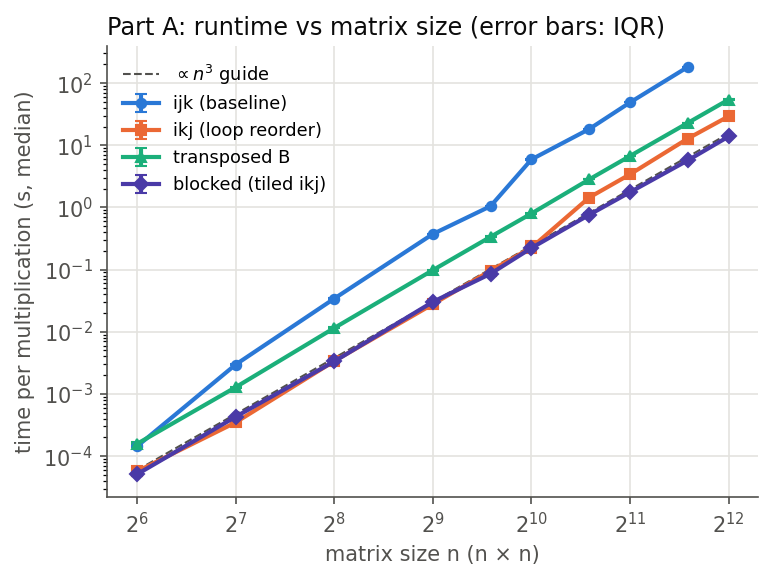
\includegraphics[width=\linewidth]{../results/figures/fig_dense_time.png}
\end{minipage}\hfill
\begin{minipage}[t]{0.495\linewidth}\centering
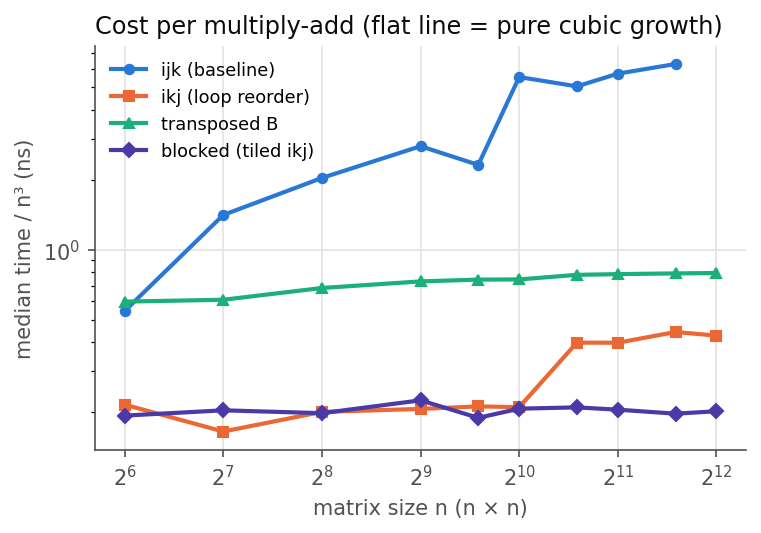
\includegraphics[width=\linewidth]{../results/figures/fig_dense_per_n3.png}
\end{minipage}
\caption{Part A. Left: median time per multiplication (log--log; the IQR bars are smaller than
the markers). Right: median time divided by $n^3$, the cost of one multiply-add; a flat line means
pure cubic growth.}
\label{fig:densetime}
\end{figure}

\begin{table}[!htbp]
\centering
\caption{Part A: speed-up over the ijk baseline (ratio of medians), throughput
$2n^3/\text{median}$, and peak working set of the process (one value per process). The peak
working set of ikj and blocked equals that of ijk within 1\,MB.}
\label{tab:speedup}
\resizebox{\linewidth}{!}{\DenseSpeedupTable}
\end{table}

\concept{Memory}
The in-place kernels follow the storage model $24n^2$ bytes plus about 4\,MB of process baseline
(231\,MB at $n=3072$ against 226\,MB predicted); transposed needs $32n^2$ (541\,MB at $n=4096$).
Under the budgets, storage limits these kernels to $n\le12\,900$ ($n\le11\,180$ for transposed),
and time limits the baseline to $n=3072$ and blocking, extrapolating its $n^3$ growth, to about
$n\approx11\,400$.

\concept{Supplementary: vectorisation versus access pattern}
With identical checksums, SSE2 vectorisation made ikj 1.25--1.65$\times$ and blocked
1.6--1.7$\times$ faster, and had no effect on transposed, whose reduction GCC does not vectorise
(Table~\ref{tab:vec}). Without vectorisation, blocking is still $18.5\times$ faster than the
baseline at $n=2048$.

\begin{table}[!htbp]
\centering
\caption{Supplementary: median time with and without loop vectorisation (same flags otherwise;
builds alternated per configuration; 5 repetitions). Raw data:
\texttt{results/supplementary/vectorization.csv}.}
\label{tab:vec}
\small\VecTable
\end{table}

\subsection{Part B: sparse versus dense}

\concept{Matched comparison}
On the same uniform inputs (Table~\ref{tab:sparse}, Figure~\ref{fig:sparsetime}) the dense time is
flat while the CSR time grows with density. CSR was faster than the blocked kernel up to 25\,\%
density and slower at 50\,\% and 100\,\%, at both sizes, with or without the conversions.

\begin{table}[!htbp]
\centering
\caption{Part B, uniform inputs: nonzeros, output density, median CSR multiplication time, CSR time
including the conversions (dense$\to$CSR of $A$ and $B$ plus CSR$\to$dense of $C$, summed
explicitly), and the dense kernels on the same logical inputs. $^\dagger$Speed-up = blocked /
CSR multiplication (both medians). nnz(B) equals nnz(A) by construction.}
\label{tab:sparse}
\resizebox{\linewidth}{!}{\SparseTable}
\end{table}

\begin{figure}[!htbp]
\centering
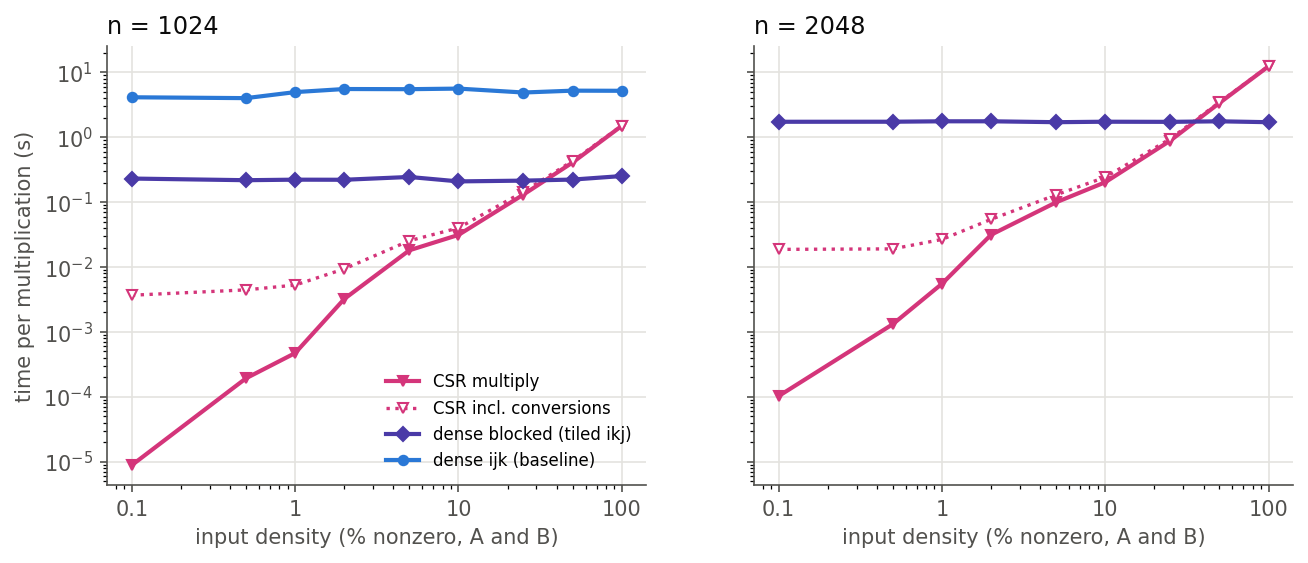
\includegraphics[width=0.97\linewidth]{../results/figures/fig_sparse_time.png}
\caption{Part B: median time per multiplication against input density, for the same logical
inputs. The dotted line adds the separately measured conversion times to the CSR multiplication.}
\label{fig:sparsetime}
\end{figure}

\concept{Conversion costs}
Converting $A$ and $B$ to CSR scans $2n^2$ entries (2.7--20\,ms at $n=1024$) and converting $C$
back costs 1--2.6\,ms (Table~\ref{tab:sparsecost}). At 0.1--0.5\,\% density the conversions take
13--420$\times$ longer than the multiplication, yet CSR with conversions is still $63\times$
($n=1024$) and $93\times$ ($n=2048$) faster than blocking at 0.1\,\%; from 2--5\,\% on the
multiplication dominates.

\begin{table}[!htbp]
\centering
\caption{Part B, uniform inputs: CSR cost breakdown (medians), time per scalar product
($\text{multiply time}/W$, with $W=\sum_k\mathrm{nnz}(A_{:,k})\,\mathrm{nnz}(B_{k,:})$), peak
working set, and the analytical CSR storage of $A$, $B$ and $C$.
$^\ast$Process of the main run, which after the multiplications also expands $A$ and $B$ to
dense arrays to time the conversions (one value per process). ``CSR only'': median over five
separate processes of the multiplication alone (\texttt{results/supplementary/sparse\_memory.csv}).}
\label{tab:sparsecost}
\resizebox{\linewidth}{!}{\SparseCostTable}
\end{table}

\concept{Output fill-in and cost per product}
The product is much denser than the inputs and its density depends on $n$ (Figure~\ref{fig:fill},
left): 1\,\% inputs give 9.7\,\% output density at $n=1024$ and 18.5\,\% at $n=2048$, and from
5\,\% on $C$ is practically dense, following the model $1-(1-d^2)^n$. The CSR time per scalar
product (right) is 4--12\,ns at densities $\le5\,\%$ and falls to 1.4--1.7\,ns at high density,
still about 7$\times$ the 0.21\,ns of a blocked multiply-add.

\begin{figure}[!htbp]
\centering
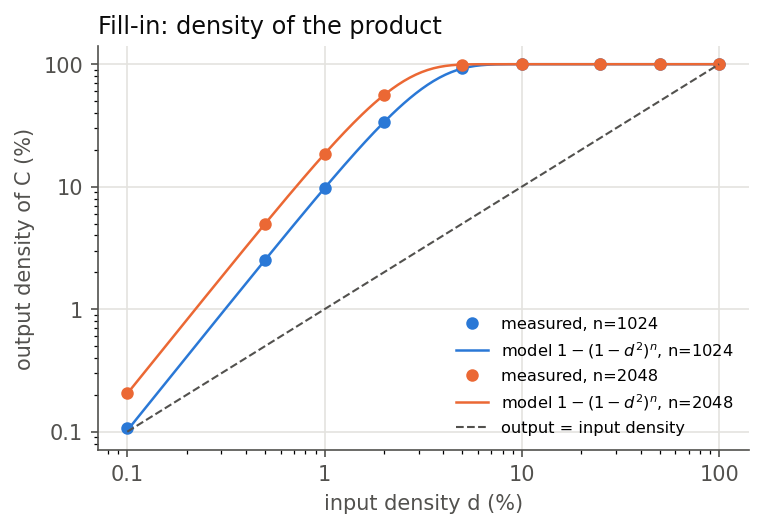
\includegraphics[width=0.43\linewidth]{../results/figures/fig_sparse_fill.png}\hfill
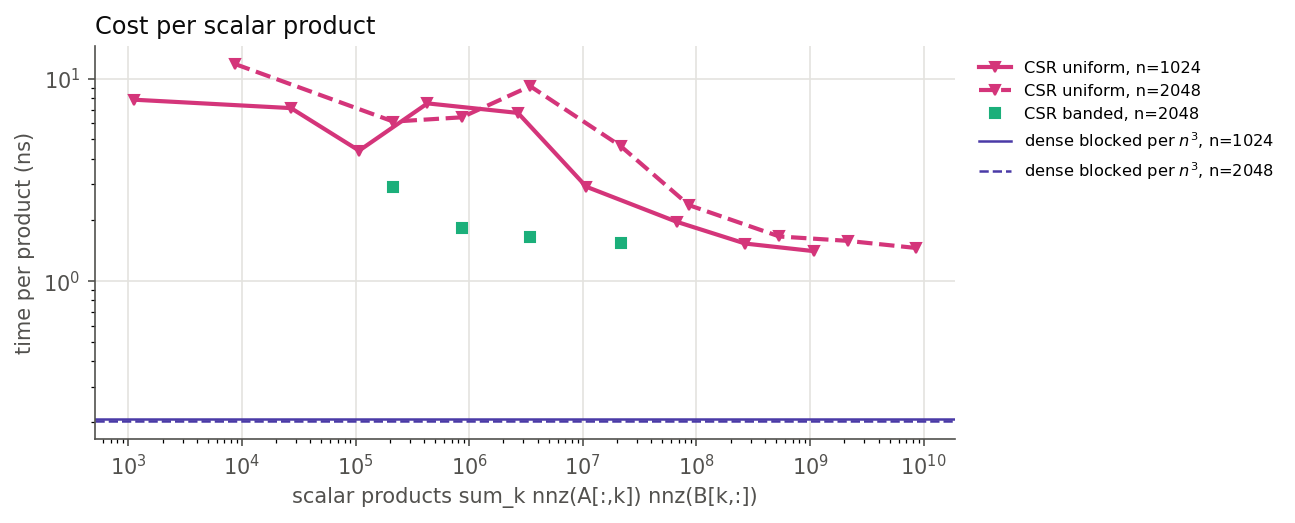
\includegraphics[width=0.55\linewidth]{../results/figures/fig_sparse_per_product.png}
\caption{Left: density of the product against the input density, with the model for independent
uniform inputs. Right: CSR time per scalar product against the number of products $W$; the
horizontal lines are the blocked kernel's time per multiply-add (median$/n^3$).}
\label{fig:fill}
\end{figure}

\concept{Memory}
The CSR multiplication alone follows the storage model of $A$, $B$ and $C$ plus the 4\,MB process
baseline (Figure~\ref{fig:sparsemem}); across its five processes the peak working set varied by
at most 12\,KB (0.2\,\%). Because $C$ fills in, CSR needed less memory than the blocked kernel up to 25\,\% density,
about the same at 50\,\%, and more at 100\,\%, where it stores 12 bytes per entry against 8.

\begin{figure}[!htbp]
\centering
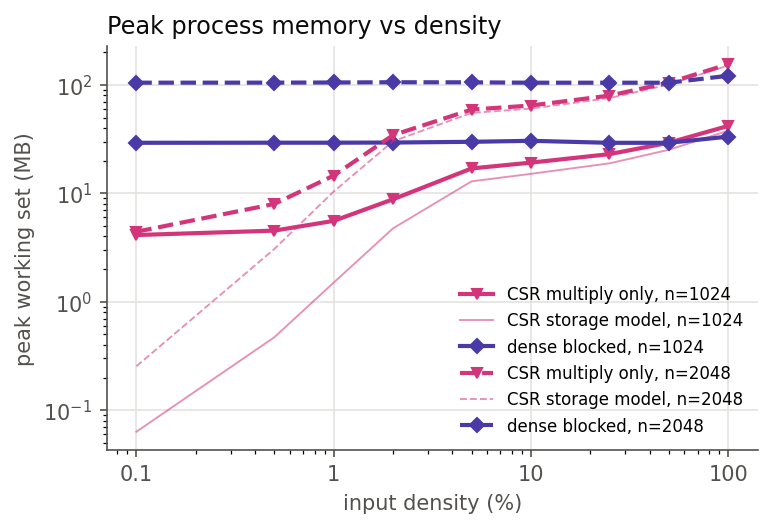
\includegraphics[width=0.62\linewidth]{../results/figures/fig_sparse_memory.png}
\caption{Peak working set of the CSR multiplication alone (median of five processes, without
conversions) and of the blocked kernel on the same inputs, with the CSR storage model of $A$, $B$
and $C$.}
\label{fig:sparsemem}
\end{figure}

\concept{Structure}
Banded and uniform inputs with the same $n=2048$, density and nnz have the same number of scalar
products within 0.5\,\% (Table~\ref{tab:structure}), but the banded products are 5--14$\times$
sparser and the CSR multiplication is 2.1--5.6$\times$ faster (1.5--2.9 instead of
4.6--9.2\,ns per product).

\begin{table}[!htbp]
\centering
\caption{Part B, $n=2048$: uniform versus banded inputs with the same density and nnz.
``Products'' is $W=\sum_k \mathrm{nnz}(A_{:,k})\,\mathrm{nnz}(B_{k,:})$.}
\label{tab:structure}
\small\StructureTable
\end{table}

\concept{Largest feasible sizes}
At 0.1\,\% density the blocked kernel took 112\,s at $n=8192$ and was not attempted at $n=16384$,
whose storage model (6.4\,GB) exceeds the budget; CSR multiplied the same $n=8192$ inputs in
4.6\,ms and reached $n=32768$ in 0.30\,s with 447\,MB (Table~\ref{tab:large},
Figure~\ref{fig:large}). At 1\,\% density the output fills in (80.6\,\% at $n=16384$, 2.7\,GB),
and the CSR run at $n=32768$ exceeded the 4\,GB budget. Table~\ref{tab:limits} summarises the limits.

\begin{table}[!htbp]
\centering
\caption{Part B beyond the dense budget (uniform inputs). The CSR peak working set at $n=4096$
includes the dense buffers of the conversion timing (conversions were timed only for
$n\le4096$). ``memory limit'' at blocked $n=16384$: not attempted, storage model above 4\,GB.}
\label{tab:large}
\resizebox{\linewidth}{!}{\LargeTable}
\end{table}

\begin{figure}[!htbp]
\centering
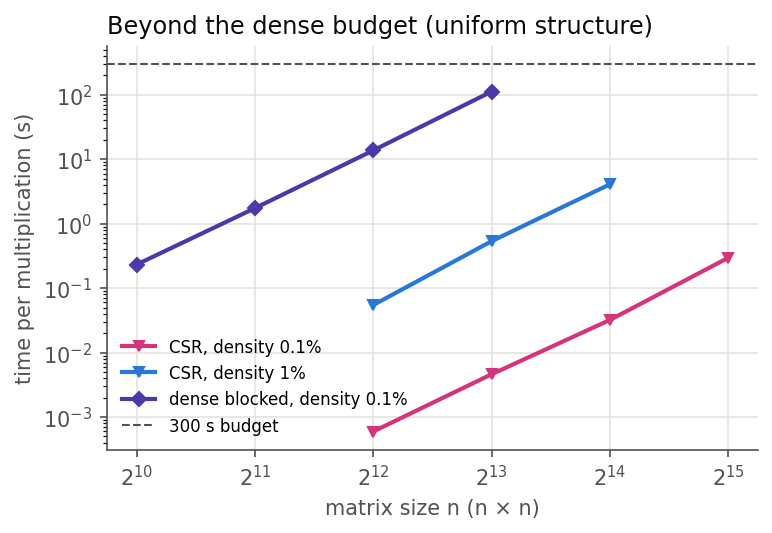
\includegraphics[width=0.62\linewidth]{../results/figures/fig_sparse_large.png}
\caption{Median time per multiplication of CSR (0.1\,\% and 1\,\% density) and of the blocked
kernel (0.1\,\%) up to the largest size that fits the budgets.}
\label{fig:large}
\end{figure}

\begin{table}[!htbp]
\centering
\caption{Largest completed size per method and the limit that stopped it
(\texttt{results/summary/limits.csv}).}
\label{tab:limits}
\small
\begin{tabularx}{\linewidth}{@{}l l r X@{}}
\toprule
Method & Input & Largest $n$ & Limit reached \\
\midrule
ijk (baseline) & dense & 3072 & $n=4096$: no multiplication within 300\,s \\
ikj, transposed, blocked & dense & 4096 & none (largest tested size) \\
blocked & uniform 0.1\,\% & 8192 & $n=16384$: storage model 6.4\,GB $>$ 4\,GB, not attempted \\
CSR & uniform 0.1\,\% & 32768 & none (largest tested size) \\
CSR & uniform 1\,\% & 16384 & $n=32768$: peak working set $>$ 4\,GB (output fill-in) \\
\bottomrule
\end{tabularx}
\end{table}

\concept{Deviations from the plan}
(i) During the first ijk run at $n=3072$ the laptop entered Modern Standby for seven minutes
(Windows Kernel-Power events 506/507); that run and the following $n=4096$ run were discarded
(\texttt{results/raw/excluded.csv}) and rerun with a keep-awake request. (ii) The session was
stopped when the laptop ran low on memory during the unrecorded attempt of blocked at $n=16384$;
the driver then gained a pre-launch check of the dense storage model against the budget, and the
remaining configurations were run with \texttt{--resume}. Each configuration runs in its own
process, so completed results were not affected.

% =====================================================================
\FloatBarrier
\section{Discussion}

\concept{Part A: what makes the optimised kernels faster}
Since the results are bitwise identical, the differences come only from how the operations are
scheduled. Reordering to i-k-j makes the inner loop stream rows of $B$ and $C$ with unit stride
and independent iterations, which lets GCC use SSE2 vectors; this sustains about 10\,GFLOP/s
while $B$ (8\,MB at $n=1024$) fits in the 16\,MB L3, but from $n=1536$ ($B=18.9$\,MB)
every row $i$ streams all of $B$ from DRAM and the cost doubles. Blocking reuses each
$64\times64$ tile of $B$ for 64 rows of $C$, so memory traffic falls by a factor of about $b$
\cite{lam} and the cost stays flat up to $n=4096$. The transposed kernel removes the strided
access too, but its inner loop is a scalar reduction that cannot be vectorised, so it is limited
by the latency of dependent additions rather than by memory: independent updates mattered more
than a contiguous layout alone.

\textbf{H1} is partly supported: the constant cost holds for blocking, and for ikj only while $B$
fits in L3; the speed-up grew with $n$, but a clear power-of-two peak appeared only at $n=1024$.
\textbf{H2} is supported in its prediction but not in its mechanism: blocking was the fastest from
$n=768$ and ikj was as fast for $n\le1024$, but the threshold was set by the whole matrix $B$
leaving the L3 cache, not by a row of $B$ leaving L2 as we expected.

Of the $27.8\times$ of blocking at $n=2048$, about $18.5\times$ remains without SIMD, so the access
pattern accounts for most of the gain. The 1.6$\times$ from 16-byte vectors is below the
theoretical factor of two, again suggesting a memory limit. Register blocking, AVX2 FMA vectors
and threads, as in optimised libraries \cite{goto}, were outside the scope of this sequential study.

\concept{Part B: optimisation effect versus sparse-storage effect}
A speed-up of CSR over the baseline mixes two effects: at $n=1024$ and 1\,\% density, the
$10\,600\times$ gain splits into $22\times$ from dense optimisation (ijk $\to$ blocked) and
$472\times$ from sparse storage (blocked $\to$ CSR). Even at 100\,\% density CSR was $3.5\times$
faster than the baseline, because Gustavson's algorithm reads $B$ in i-k-j order, but $6\times$
slower than blocking. Part~B speed-ups are therefore reported against the blocked kernel.

\concept{When the sparse representation pays off}
CSR does $W\approx n^3d^2$ products instead of $n^3$ but pays 1.4--12\,ns per product instead of
0.21\,ns, because each product needs an index load, an indirect accumulator access and a marker
test, and is not vectorised. With the high-density cost of 1.5\,ns, the break-even density is
$d\approx\sqrt{0.21/1.5}\approx37\,\%$, consistent with the measured crossover between 25\,\% and
50\,\%. \textbf{H3} is therefore supported at low density but not for the crossover, which was
higher than the ten percent we expected because the cost per product fell at high density. The
memory crossover is similar because the output fills in. Conversions matter only when the data
arrive in dense form; being $O(n^2)$ against the $O(n^3)$ dense product, they never removed the
advantage.

\concept{Density alone does not determine performance}
\textbf{H4} is supported by three results: the output density depends on $n$ as well as on the
input density; the cost per product varied by a factor of 8 between densities; and at the same
density, nnz and number of products, banded inputs produced 5--14$\times$ fewer output nonzeros
and ran up to 5.6$\times$ faster, because a product of two bands is again a band and the combined
rows of $B$ touch neighbouring accumulator entries. The CSR runtime depends on the number of
products, the number of distinct output entries and the locality of the accumulator accesses, all
of which depend on the structure. The largest feasible size is limited by output fill-in rather
than by $n^2$ storage.

\concept{Limitations}
\begin{itemize}[leftmargin=1.4em]
  \item One machine, compiler and flag set; no \texttt{-march}, so no AVX2 or FMA. The ranking
        may change with wider vectors or other cache sizes.
  \item The baseline varied between processes: on the Part~B inputs of $n=1024$ (same work) its
        median ranged from 4.0 to 5.6\,s, so speed-ups relative to it carry about $\pm15\,\%$
        uncertainty; those of the blocked kernel (209--253\,ms) much less.
  \item Synthetic uniform and banded inputs only; real sparse matrices would move the crossover.
        CSR output columns are unsorted, which some consumers would have to sort.
  \item Memory is the peak working set of the whole process, sampled every 20\,ms and
        including a 4\,MB baseline. In the main runs it is one value per process covering all
        repetitions; only the CSR-only supplementary repeats it in five processes.
  \item No hardware counters: the cache and latency explanations agree with the measurements but
        are not confirmed by miss counts.
\end{itemize}

% =====================================================================
\section{Conclusions}
\begin{titledbox}{Key findings}
On this machine and with these settings:
\begin{itemize}[leftmargin=1.2em]
  \item All optimised dense kernels gave \textbf{bitwise-identical results} to the baseline, so
        they differ only in how they use memory and the processor.
  \item \textbf{Cache blocking} was the fastest dense method (about 10\,GFLOP/s at every size,
        $31.8\times$ the baseline at $n=3072$); the baseline could not finish $n=4096$ in 300\,s.
  \item \textbf{Loop reordering} matched blocking only while $B$ fit in the L3 cache;
        \textbf{transposed} was limited by its scalar reduction. Vectorisation contributed
        1.25--1.7$\times$, the access pattern the rest.
  \item \textbf{CSR} beat the fastest dense kernel by more than two orders of magnitude at
        densities $\le1\,\%$ and by up to $2\times$ at 25\,\%, and lost from 50\,\%; conversions
        dominated up to 1--2\,\% density but never removed its advantage.
  \item The \textbf{sparse advantage depended on fill-in and structure}, not on input density
        alone, and CSR extended the largest feasible size from $n=8192$ to $n=32768$ at 0.1\,\%.
\end{itemize}
\end{titledbox}

\concept{Open questions}
Whether register blocking and AVX2/FMA change the ranking, a hardware-counter confirmation of the
cache explanations, and how the crossover moves for real sparse matrices.

% =====================================================================
\section*{Reproducibility materials}
Repository: \url{\RepoURL}. It contains the source code (\texttt{c/}; the baseline kernel body is
copied unchanged from Assignment~1, \url{\AOneURL}), the configuration
(\texttt{config/benchmark\_config.json}), the input generator with SHA-256 of every input
(\texttt{scripts/generate\_inputs.py}, \texttt{data/manifest.json}), the build, tuning, benchmark,
validation, supplementary and analysis scripts, all raw measurements (\texttt{results/raw/},
including the excluded rows and the reason, \texttt{results/tuning/},
\texttt{results/supplementary/}), and a README with exact commands and dependency versions.

\section*{Use of generative AI}
Claude Opus (Anthropic), used through Claude Code, assisted with: writing and debugging the C
kernels and the Python scripts (input generation, benchmark driver, validation, analysis and
figures); running the measurement campaign on the author's machine; and drafting and revising the
text of this report. The author defined the study, reviewed the code and checked every number in
the report against the raw data in the repository. Generated content was not used as evidence:
all results come from executing the code, and all references were checked to exist.

% =====================================================================
\begin{thebibliography}{99}\small\sloppy
\setlength{\itemsep}{1pt}
\bibitem{golub} G.~H. Golub and C.~F. Van~Loan, \emph{Matrix Computations}, 4th ed. Baltimore, MD, USA: Johns Hopkins Univ. Press, 2013.
\bibitem{drepper} U.~Drepper, ``What every programmer should know about memory,'' Red Hat, Inc., 2007. [Online]. Available: \url{https://people.freebsd.org/~lstewart/articles/cpumemory.pdf}
\bibitem{lam} M.~S. Lam, E.~E. Rothberg, and M.~E. Wolf, ``The cache performance and optimizations of blocked algorithms,'' in \emph{Proc. ASPLOS-IV}, 1991, pp.~63--74.
\bibitem{goto} K.~Goto and R.~A. van~de~Geijn, ``Anatomy of high-performance matrix multiplication,'' \emph{ACM Trans. Math. Softw.}, vol.~34, no.~3, art.~12, 2008.
\bibitem{strassen} V.~Strassen, ``Gaussian elimination is not optimal,'' \emph{Numerische Mathematik}, vol.~13, pp.~354--356, 1969.
\bibitem{gcc12} GNU Project, ``GCC 12 Release Series: Changes, New Features, and Fixes,'' 2022. [Online]. Available: \url{https://gcc.gnu.org/gcc-12/changes.html}
\bibitem{saad} Y.~Saad, \emph{Iterative Methods for Sparse Linear Systems}, 2nd ed. Philadelphia, PA, USA: SIAM, 2003.
\bibitem{gustavson} F.~G. Gustavson, ``Two fast algorithms for sparse matrices: Multiplication and permuted transposition,'' \emph{ACM Trans. Math. Softw.}, vol.~4, no.~3, pp.~250--269, 1978.
\bibitem{smmp} R.~E. Bank and C.~C. Douglas, ``Sparse matrix multiplication package (SMMP),'' \emph{Advances in Computational Mathematics}, vol.~1, pp.~127--137, 1993.
\bibitem{davis} T.~A. Davis, \emph{Direct Methods for Sparse Linear Systems}. Philadelphia, PA, USA: SIAM, 2006.
\bibitem{higham} N.~J. Higham, \emph{Accuracy and Stability of Numerical Algorithms}, 2nd ed. Philadelphia, PA, USA: SIAM, 2002.
\bibitem{scipy} P.~Virtanen \emph{et al.}, ``SciPy 1.0: Fundamental algorithms for scientific computing in Python,'' \emph{Nature Methods}, vol.~17, pp.~261--272, 2020.
\bibitem{amd} Advanced Micro Devices, ``Software Optimization Guide for AMD Family 19h Processors,'' Pub. no. 56665, 2020.
\bibitem{psutil} G.~Rodola, ``psutil documentation,'' 2026. [Online]. Available: \url{https://psutil.readthedocs.io/}
\end{thebibliography}

\end{document}
